\documentclass[11pt, a4paper]{article}
\usepackage[T2A]{fontenc}
\usepackage[utf8]{inputenc}
\usepackage[bulgarian]{babel}

%% Sets page size and margins
\usepackage[a4paper,top=3cm,bottom=3cm,left=3cm,right=3cm,marginparwidth=1.75cm]{geometry}

%% Useful packages
\usepackage{amsmath, amssymb, amsthm,calc,mathabx}
\usepackage{systeme}
\usepackage{graphicx}
\usepackage[colorinlistoftodos]{todonotes}
\usepackage[colorlinks=true, allcolors=black]{hyperref}
\usepackage{wrapfig,lipsum,booktabs}
\usepackage{enumitem}
\usepackage{float}
\usepackage{fmtcount}
\usepackage{multicol}
\usepackage{breqn}
\usepackage{setspace}
\usepackage{hyperref}
\usepackage{mathtools}
\usepackage {tikz}
\usetikzlibrary {positioning}
\usetikzlibrary{shapes.geometric}
\graphicspath{
	{Graphics/}
	{Graphics/BackupFunction/}
}
\newtheorem{theorem}{Theorem}

\newtheorem{lemma}{Lemma}
\newtheorem{prop}{Property}
\newtheorem*{remark}{Remark}

\theoremstyle{definition}
\newtheorem{definition}{Дефиниция}

\setlength{\columnsep}{1cm}
\setlength{\parindent}{1em}

\newcommand\blfootnote[1]{%
	\begingroup
	\renewcommand\thefootnote{}\footnote{#1}%
	\addtocounter{footnote}{-1}%
	\endgroup
}

\begin{document}
\begin{titlepage}
	\newcommand{\HRule}{\rule{\linewidth}{0.5mm}}
	\centering
	\textsc{\LARGE УК БАН '20}\\
	
\includegraphics[width=0.5\textwidth]{Uchimi_logo}\\
	\HRule\\[1 cm]
	{\huge\bfseries Устойчиви Стратегии за Архивиране}\\[1 cm]
	\HRule\\
	\vfill
			\Large
			\textit{Автор:}
			 \textsc{Никола Стайков}\\
             \vspace{2cm}
			\Large
			\textit{Ментор:}
            \textsc{Явор Папазов}
    \vfill	
	{\large\today}   
	\vfill
\end{titlepage}

\tableofcontents
\newpage
\begin{abstract}
		Архивите представляват резервни копия на данни, които да бъдат възстановени в случай на злополука. Те са основното средство за защита срещу рансъмуер и други видове вируси, както намаляват рисковете от критични щети в случай на природни бедствия. На свой ред обаче могат да представляват съществен разход за големите компании поради огромното количество данни, които трябва да бъдат подсигурени. Това на свой ред поражда нуждата те да бъдат внимателно планирани. Настоящият проект разразглежда модел за архивиране на данни, състоящ се от пълни и инкрементални архиви, изчислявайки очакваната цена за възстановяване на данните и цената на съхранение. Процесът по възстановяване е пресъздаден и анализиран чрез визуализация на python и Монте Карло симулация. Моделът намира оптимална стратегия за архивиране при предварително въведени параметри, характеризиращи работата на конкретния клиент.
\end{abstract}

\section{Въведение}
		Настоящият проект изгражда теоретичен математически модел с цел намирането на оптимална стратегия за архивиране. Моделът включва два вида архиви, пълни и инкрементални. Параметрите, които оптимизираме, са интервалите в дни между видовете архиви. Структурата от архиви между два пълни архива образува цикъл, който се повтаря неопределено. Той се дефинира изцяло от два интервала - между пълните и между инкременталните архиви. Получените резултати се базират на два основни компонента- възможността за провал при възстановяваване на данните (различна за видовете архиви) и цената за съхранение на данните. Ефектите на двата компонента се изчисляват самостоятелно като след това се обединяват посредством константа, показваща отношението между цената на данните и техния размер. Подобни модели са правени и в миналото \cite{qian2010optimal}, \cite{nakamura2003optimal}, но те разглеждат само цената за съхранение, при неконстантна скорост на генериране на данни. Там интервалът между два последователни архива не е константен. За пълното разбиране на проекта са нужни базови знания по статистика и вероятности, използвани са стандартни означения и дефиниции.

\section{Теоретична постановка}
	Настоящият модел е създаден с цел да изчисли и оптимизира очакваната цена като сума на два компонента, цена на възстановяване и цена на съхранение. Двата за разгледани поотделно като очакваната цена за всеки от тях е изчислена при различни стратегии на архивиране. Моделът обединява двата компонента чрез безразмерна величина, отразяваща отношението между стойността на генерираните данни и цената за тяхното съхранение.
	\subsection{Възстановяване}
		Ще разглеждаме архивът като структура от данни със следните компоненти:
		$$
		b
		\begin{cases}
		d \text{: датата на създаването на архива като разлика в дни от първия архив}\\
		p \text{: вероятността възстановяването да е неуспешно}\\
		r \text{: цената за опит за възстановяване}
		\end{cases}
		$$
		Разгледани са два вида архиви:
		\begin{enumerate}
			\item Пълен архив: запазва копие на цялата база данни до момента на създаване
			\item Инкрементален архив: запазва само промените спрямо последния архив
		\end{enumerate}
		Архивите от конкретен вид имат обща вероятност за провал и цена за опит за възстановяване. \par
		За да може един инкрементален архив да е успешен, трябва всички инкрементални архиви преди него до успешен пълен архив също да са успешни, както и самият пълен архив.\par
		Важно е да се отбележи, че цената на данните в случая не съвпада с пазарната им такава. Това е така поради субективната им важност за компанията. Това е и причината в описания модел цената на данните да се разглежда като вечно увеличаваща се величина и за целите на изследването "скоростта на работа" на компанията се счита за константа. Ще я означим с $w$.\par
		Цената на процеса по възстановяване ще разглеждаме като сума от два фактора:
		\begin{enumerate}
			\item Цената на изработването на загубените данни, означена с $W$
			\item Цената на процеса по възстановяването, означена с $R$.
		\end{enumerate}
		Дефинираме $W = \Delta t.w$, където с $\Delta t$ означаваме разликата в дни между датата на създаване на последния успешно възстановен архив и датата на възстановяване, и $R = \sum_{i=1}^{n} r_i$, където броят опити за възстановяване е $n$.
		Нека разликата в дни между първия направен архив и датата на възстановяване е $T$. В случай, че никой от пълните архиви не се окаже успешен, въвеждаме променлива $W_T$, съответстваща на цената на преработване на всички съществуващи файлове. Ясно е, че $W_T>T.w$\par
	\subsection{Съхранение}
		
			\subsubsection{Пълни архиви}
				Когато разглеждаме само пълни архиви, моделът е разпределение на Бернули с краен брой опити, а именно броят пълни архиви. Спираме, когато успеем да намерим успешен архив, започвайки от последния и вървейки към първия. Да дефинираме свойствата на пълен архив($B_F$):
				$$
				B_F
				\begin{cases}
				p_F: \text{вероятността за провал}\\
				r_F: \text{цената за опит за възстановяване}\\
				t_F: \text{дните между два последователни пълни архива}\\
				\end{cases}
				$$
				Нека $k$ е броят пълни архиви направени преди деня на атаката. Тогава:
				$$
				k = \left \lfloor{\frac{T}{t_F}}\right \rfloor + 1
				$$
				Сега можем да дефинираме очакваната цена на възстановяване:
				\begin{equation}
					\label{eq:1}
					E(T) = p_F^{k}\left(W_T + k.r_F\right) + \displaystyle \sum_{i=0}^{k-1} 	(1-p_F).p_F^{i}\left( \left (\left\{ \frac{T}{t_F}\right \} + i\right)t_F.w + (i+1).r_F \right )
				\end{equation}
				Направените изчисления са ключови поради невъзможността инкременталните архиви да бъдат възстановени без работещ пълен архив и следователно намирането на такъв е първият ни приоритет. Сега можем да разгледаме инкременталните архиви при работещ пълен архив.
			\subsubsection{Инкрементални архиви с работещ пълен архив}
				Ще разгледаме случая, когато имаме работещ пълен архив и се опитваме да възстановив допълнителни данни чрез инкрементални архиви.\\
				\begin{tikzpicture}
				[every node/.style={inner sep=0pt}]
				\node (1) [circle, minimum size=50.0pt, fill=teal, line width=0.625pt, draw=black] at (50.0pt, -130pt)  {};
				\node (2) [circle, minimum size=31.25pt, fill=lime, line width=0.625pt, draw=black] at (135pt, -130pt)  {};
				\node (3) [circle, minimum size=31.25pt, fill=lime, line width=0.625pt, draw=black] at (220pt, -130pt)  {};
				\node (4) [circle, minimum size=31.25pt, fill=lime, line width=0.625pt, draw=black] at (305pt, -130pt)  {};
				\node (5) [circle, minimum size=50.0pt, fill=teal, line width=0.625pt, draw=black] at (390pt, -130pt)  {};
				\draw [line width=0.625, ->, >=latex, color=black] (1) to  (2);
				\draw [line width=0.625, ->, >=latex, color=black] (2) to  (3);
				\draw [line width=0.625, ->, >=latex, color=black] (3) to  (4);
				\draw [line width=0.625, ->, >=latex, color=black] (4) to  (5);
				\end{tikzpicture}\\
				Нека дефинираме свойствата на инкременталните архиви ($B_I$) по подобен начин:
				$$
				B_I
				\begin{cases}
					p_I: \text{вероятността за провал}\\
					r_I: \text{цената за опит за възстановяване}\\
					t_I: \text{дните между два последователни инкрементални архива}\\
				\end{cases}
				$$
		\newpage
				Нека с $T_F$ да означим разликата в дни между денят на атаката и датата на успешния пълен архив и с $l$ да означим броят инкрементални архиви, които трябва да разгледаме. Имаме две опции за $l$ в зависимост от това дали последният пълен архив е бил успешно възстановен:
				$$
				l=
				\begin{cases}
				\left\lfloor \frac{T_F}{t_I}\right \rfloor \text{, ако } T_F<t_F\\
				\left\lfloor \frac{t_F}{t_I}\right \rfloor -1 \text{, ако } T_F>t_F\footnotemark\\
				\end{cases}
				$$
				\footnotetext{Можем да опитваме да възстановим само инкрементални архиви предхождащи следващият пълен архив}
				Да отбележим, че това последният пълен архив да е успешен е еквивалентно на $T_F<t_F$.\par
				Сега сме в точно обратната ситуация спрямо миналата част. Процесът по възстановяване на инкрементални архиви продължава докато не се натъкнем на провал, тъй като това би означавало, че всички следващи инкрементални архиви също са неизползваеми. С това намаляме $W$, тъй като в началната позиция сме готови да преработим данните до датата на успешния пълен архив. Сега сме готови да изчислим очакваната цена:
				\begin{equation}
					\label{eq:2}
					f(T_F) = (1-p_I)^l.((T_F-t_I.l).w + r_I.l) + \displaystyle \sum_{i=0}^{l-1} (1-p_I)^{i}.p_I((T_F-t_I.i)w + r_I.(i+1))
				\end{equation}
				Сега знаем колко ще намалее цената на възстановяването, когато използваме инкрементални архиви, и можем да построим цялостния модел, използвайки уравнения \ref{eq:1} и \ref{eq:2}.
			\subsubsection{Очаквана цена на възстановяване}
				Към всяко събираемо в уравнение \ref{eq:1} трябва да добавим ефектът на инкременталните архиви и получаваме нови събираеми от вида:
				$$
				P(W + R),
				$$
				където $P$ е вероятността определена комбинация от събития да се случи, $W$ е цената на данните, които трябва да бъдат създадени наново, а $R$ е цената на процесът по възстановяването. Инкременталните архиви намаляват цената на данните, които трябва да бъдат създадени наново, но увеличават $R$. Както споменахме по-горе, има само един случай, вкойто броят инкрементални архиви, които трябва да имаме предвид е различен и той е именно този, в който последният пълен архив е възстановен успешно. Ако $i$-тият пълен архив е успешен\footnote{Това съответства на $i-1$-вото събираемо в сумата от уравнение \ref{eq:3}}:
				$$
				T_F=t_F\left(\left\{ \frac{T}{t_F} \right\} + i - 1\right)
				$$
				Комбинирайки уравнения \ref{eq:1} и \ref{eq:2} получаваме:
				\begin{equation}\label{eq:3}
				F(T) = p_F^{k}(W_T+k.r_F) + \displaystyle\sum_{i=0}^{k-1}(1-p_F).p_F^{i}\left(f(T_F) + (i+1).r_F\right)
				\end{equation}
				Използвайки уравнения \ref{eq:1} и \ref{eq:3}, можем да построим графика на очакваната цена с и без използването на инкрементални архиви.
				\begin{figure}[H]
					\begin{minipage}{1.0\textwidth}
						\centering
						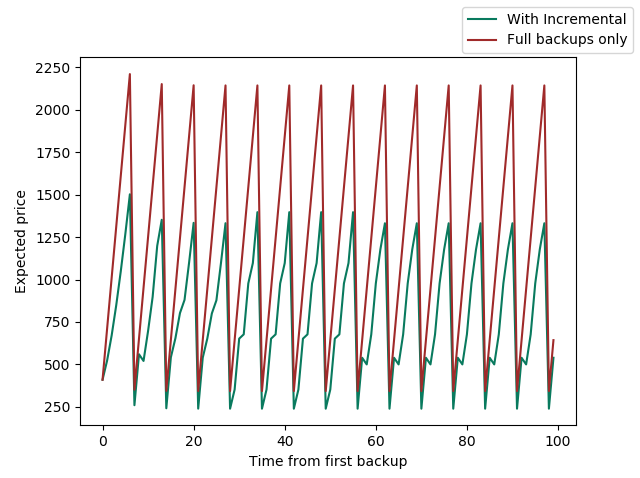
\includegraphics[width=0.7\textwidth]{Weekly_full.png}
						\caption{Full only and Whole model}\label{Fig:FullWeekly}
					\end{minipage}
				\end{figure}
			\subsubsection{Симулация Монте Карло}
				Направена бе симулация от тип Монте Карло на python, която генерира случайни процеси на възстановяване на данни с описаната структура на архивите. Цената на възстановяването беше направена на графика спрямо датата на атаката:
				\begin{figure}[H]
					\begin{minipage}{1.0\textwidth}
						\centering
						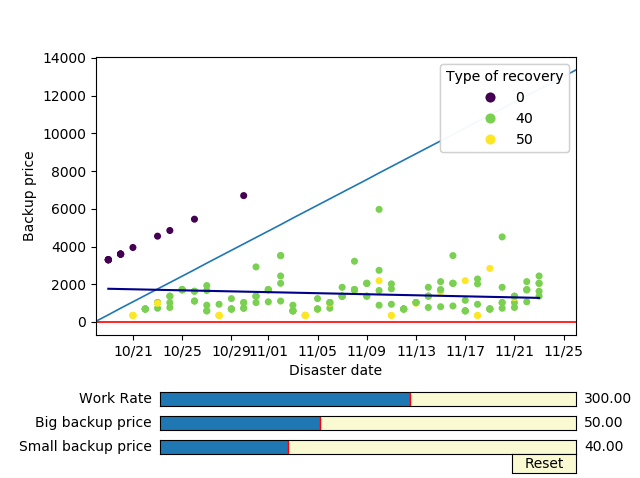
\includegraphics[width=0.7\textwidth]{Weekly_full_carlo.png}
						\caption{Симулация Монте Карло}\label{Fig:MonteCarlo}
					\end{minipage}
				\end{figure}
				\blfootnote{Във фигура \ref{Fig:FullWeekly} и фигура \ref{Fig:MonteCarlo} данните са за седмичен пълен архив и ежедневен инкрементален}
				Цветовете във фигура \ref{Fig:MonteCarlo} показват вида на последния успешно възстановен архив, пълен, инкрементален или несъществуващ.
				\newpage
				Линейна регресия на данните беше генерирана, която показва как ефектът от начално неподсигурените данни намалява с времето, тъй като цената при провал се изчилсява като цената за преработването на всички данни, които компанията е генерирала.
		\subsection{Цена на съхранение}
			Цената на съхранение се генерира от вече създадените архиви като за всеки индивидуално зависи от вида му и датата на създаване. За всяка от стратегиите изчисляваме цената за съхранение на данни от $t$ дни, поради съображения, че размерът на важните данни, които бихме съхранявали по-дълго, е незначителен. Цената за съхранение на определено количество  данни за един ден ще означим със $s$. За целите на модела приемаме, че тя е пропорционална на цената за създаването на данните. За да отразим това взаимоотношение въвеждаме безразмерната величина $c = \dfrac{s}{w}$.\par
			Размерът на пълен архив, направен в дадена времева точка $x$ има размер $x.w$, където $w$ e скоростта на работа. Цената за съхранението му за ден е $s$ и сме го съхранявали $T-x$ дни, поради което конкретният пълен архив е генерирал цена за съхранение $xw(T-x)s = cw^2x(T-x)$   За дадена стратегия цикъл ще наричаме периода между два пълни архива. Размерът на запазените данни в рамките на един цикъл е 
			\begin{equation}
				t_F
			\end{equation}
		\subsection{Резултати}
			Беше построен модел за изчисляване на очакваната цена при възстановяване на данни. Нещо повече, ефектът от инкременталните архиви беше показан в сравнение със стратегия използваща само пълни архиви. Беше направена и анализирана симулация от тип Монте Карло, коятодемонстрира реалния процес на възстановяване.
	\section{Бъдещо развитие}
		Авторът разглежда няколко посоки за бъдещото развитие на проакта, а именно:
		\begin{itemize}
			\item разглеждане на неконстантна скорост на работа за модела за архивиране
			\item разширяване на модела за откуп в посока описване на по сложни начини за разпространение на рансъмуера.
			\item използване на резултатите и базите данни на подобни проучвания с цел подкрепянето на модела с реални данни.\cite{paquet2019ransomware}
			\item използване на динамичен модел за оценка на откупа
		\end{itemize}
	\section{Благодарности}
		Искам да благодаря на своя ментор, Явор Папазов, и на Константин Делчев за безотказната помощ в избора на темата на проекта и последващото му развитие, за снабдяването ми с всички нужни материали за запознаването ми с темата, както и за изслушването на въпросите ми. Искам също да благодаря на Станислав Харизанов за професионалните съвети.
\nocite{*}
\bibliographystyle{unsrt}
\bibliography{Bibliography}
\end{document}